\chapter{Experiments and Evaluation}
\label{evaluation}
% DELETEME: The evaluation chapter is one of the most important chapters of your work. Here, you will prove usability/efficiency of your approach by presenting and interpreting your results. You should discuss your results and interpret them, if possible. Drawing conclusions on the results will be one important point that your estimators will refer to when grading your work.

This chapter serves as a presentation of our the dataset used in our experiments, and their output, after which is discussed if it has met the expectations and the approach was efficient in providing a solution for the camera placement optimisation problem.

\section{Experiments}
In this thesis, two different experiments were conducted in order to evaluate the performance loss of cameras. What is more, with the help of heatmaps and using the metrics M1 and M2 we are able to define an optimal camera position. The experiments aim to check if problems from \ref{problem_analysis} are handled efficiently by the proposed strategy. In the next subsections, we inform about the laptop used for our simulations and explain into details each experiment. Afterwards, we discuss the results and the efficiency of our metrics.

\subsection{Technical specifications}
The following list contains technical specifications of the machine, which all experiments were simulated on:
\begin{itemize}
    \item \textbf{Processor} - Intel Core i7-10750H CPU 2.60GHz
    \item \textbf{RAM} - 16 GB DDR5
    \item \textbf{GPU} - NVIDIA GeForce RTX 3060 6 GB
    \item \textbf{SSD} - 1 TB
\end{itemize}

\newpage
\subsection{First experiment - change height and angle of camera}
The main objective of our first experiment is to evaluate the performance of cameras at different height, because we concluded in Chapter \ref{problem_analysis} that in the found literature there is little information about which height is optimal for traffic surveillance. We use heatmaps to present the highest occlusion degree for each spawn point. Additionally, our metric M2 is applied in order to see what part occlusion situations were from all cases and choose positions which has scored lower values. During the execution of simulations, we rely on a camera with the following configurations:
\begin{itemize}
    \item FoV (horizontal angle) = $80^{\circ}$
    \item Resolution = $1280\times720$ pixels or also known as 720p
\end{itemize}
The reason for our horizontal angle is that we wanted to cover as much as possible from our region of interest and an average traffic surveillance camera on the market has a horizontal field of view $70^{\circ} - 110^{\circ}$. In a real-world scenario, a wider field of view will cause a fisheye effect\footnote{When an image is distorted by stretching the picture around a rounded camera lens} to occur and has to be taken into account. However, in our experiments the conditions are ideal and we do not apply image distortion. We have 8 enumerated positions for the camera, which can be seen in Figure \ref{fig:positions_enumerated}, where we place it at a pre-defined height. On each of these spawn locations for our sensor, we define 6 levels for the height beginning at 5 meters and going to 10 meters with a 1-meter step. This results in 48 simulations, where we set $0^{\circ}$ for the tilt angle at 5 meters, $-10^{\circ}$ at 6 meters and then go to $-30^{\circ}$ at 10 meters with a $-5^{\circ}$ step. In this way we guarantee that the camera has approximately the same sight over the vehicles and the blind spot under the sensor does not increase. The region of interest is limited by the red lines in Figure \ref{fig:positions_enumerated} and is used in each of the two experiments.

During each simulation, we generate a list with waypoints for the target vehicle that are 3 meters apart and one for the occluder, but with 1-meter distance between spawn points. We decided to use Seat Leon (see Fig. \ref{fig:seat_leon}) as a target and Jeep Wrangler Rubicon (see Fig. \ref{fig:jeep_wrangler}) as an occluder for our scenarios, because in an urban area people mainly use normal cars or SUVs for their transportation needs, and therefore it is more often the case that an occlusion-prone situation between these two types of vehicles arises. In our second experiment we consider pairs of vehicles of different type in order to broaden the variety of occlusions.

\begin{figure} [h!]
    \centering
    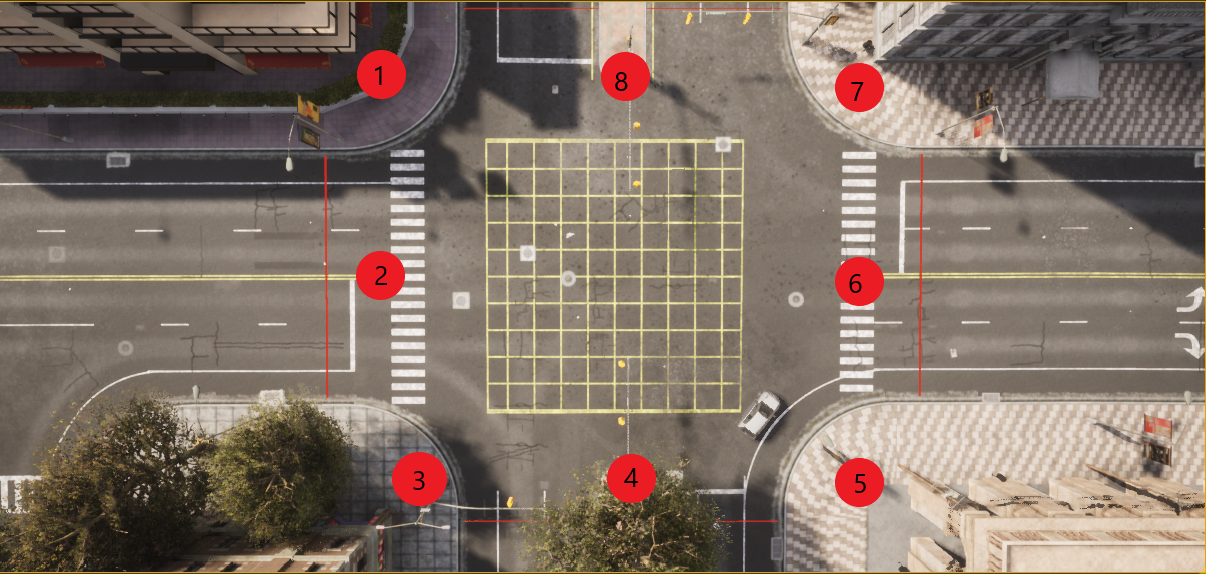
\includegraphics[width=0.90\textwidth]{images/positions_numerated.png}
    \caption[Enumerated camera positions]{This image shows the number of each camera's position used in our simulations.}
    \label{fig:positions_enumerated}
\end{figure}

\newpage
\subsection{Second experiment - change threshold for target vehicle recognition}
In our second experiment our goal is to observe how strong the occlusion is when there are different types of vehicles. Here we use the same parameters for the camera, but this time it is placed only at 8 meters above the ground. The reason behind this decision is that this value is approximately in the middle between the range of values we used in the previous experiment, and also we have mentioned in Section \ref{main_problems} that the minimum for an ideal height is exactly 8 meters. Furthermore, we guarantee same conditions for all sensor positions by setting their tilt angle at $-20^{\circ}$ in order to have an accurate comparison between each one of them. For this scenario, we use three pairs of vehicles and execute a simulation for each camera position, which comprises a total of 18 simulations, 6 of which are also part of the first experiment. Moreover, we decided to not consider positions 4 and 8 here, because their view is obstructed by the traffic lights and signs on them, therefore their range of view is limited.

For this experiment we rely on the pairs:
\begin{itemize}
    \item Seat Leon and Jeep Wrangler Rubicon
    \item Ford Mustang and Mercedes Sprinter (see Figures \ref{fig:ford_mustang} and \ref{fig:mercedes_sprinter})
    \item Ambulance truck (see Fig. \ref{fig:ambulance}) and Mercedes Sprinter
\end{itemize}
Our idea is to reproduce three possible scenarios in a traffic, in which we have a normal car and SUV, a normal car and a large van, as well as two large-sized vehicles. In this way, we can ensure that a variety of vehicles' sizes are covered by this study. Important to mention is that the distance between target spawn points is again set to 3 meters. 

For the purpose of assessing the optimal camera locations we apply our M1 metric for a priori specified threshold. In the real world it is vital for a camera to miss as little as possible objects, which were hidden due to other large-sized vehicles. Therefore, we set an occlusion tolerance threshold, after which the target vehicle is no more detectable, to 50\%, 75\% and 90\%. By implementing this constraint, we can conclude from the score of our metric how many occlusions from all the detected ones could actually blind the camera. Finally, we choose these positions, which output the lowest values. Apart from the metric, heatmaps display again the maximum occlusion degree for each target position, which was visible for the sensor.


%###################################################################################
%###################### Results             ########################################
%###################################################################################
\section{Results}\label{results}
In the heatmaps and tables below, we can inspect the results from both experiments. In order to maintain a well-arranged visualisation of the output, we are going to present only the heatmaps for 5 and 10-meter height and compare the impact of increasing elevation on the maximum occlusions. For our second experiment, we will visualise the results from cameras placed at 8 meters above the road. The other heatmaps are placed in the appendix, if one wants to analyse them.

\subsection{First experiment}

\begin{figure}[!htb]
\minipage{0.5\textwidth}
  \includesvg[width=\linewidth]{images/position0/pos0_5m.svg}
  \caption{Pos.1 at 5 m height}\label{fig:pos1_5m}
\endminipage\hfill
\minipage{0.5\textwidth}
  \includesvg[width=\linewidth]{images/position0/pos0_10m.svg}
  \caption{Pos.1 at 10 m height}\label{fig:pos1_10m}
\endminipage\hfill
\end{figure}

\begin{figure}[!htb]
\minipage{0.5\textwidth}
  \includesvg[width=\linewidth]{images/position1/pos1_5m.svg}
  \caption{Pos.2 at 5 m height}\label{fig:pos2_5m}
\endminipage\hfill
\minipage{0.5\textwidth}
  \includesvg[width=\linewidth]{images/position1/pos1_10m.svg}
  \caption{Pos.2 at 10 m height}\label{fig:pos2_10m}
\endminipage\hfill
\end{figure}

\begin{figure}[!htb]
\minipage{0.5\textwidth}
  \includesvg[width=\linewidth]{images/position2/pos2_5m.svg}
  \caption{Pos.3 at 5 m height}\label{fig:pos3_5m}
\endminipage\hfill
\minipage{0.5\textwidth}
  \includesvg[width=\linewidth]{images/position2/pos2_10m.svg}
  \caption{Pos.3 at 10 m height}\label{fig:pos3_10m}
\endminipage\hfill
\end{figure}

\begin{figure}[!htb]
\minipage{0.5\textwidth}
  \includesvg[width=\linewidth]{images/position3/pos3_5m.svg}
  \caption{Pos.4 at 5 m height}\label{fig:pos4_5m}
\endminipage\hfill
\minipage{0.5\textwidth}
  \includesvg[width=\linewidth]{images/position3/pos3_10m.svg}
  \caption{Pos.4 at 10 m height}\label{fig:pos4_10m}
\endminipage\hfill
\end{figure}

\begin{figure}[!htb]
\minipage{0.5\textwidth}
  \includesvg[width=\linewidth]{images/position4/pos4_5m.svg}
  \caption{Pos.5 at 5 m height}\label{fig:pos5_5m}
\endminipage\hfill
\minipage{0.5\textwidth}
  \includesvg[width=\linewidth]{images/position4/pos4_10m.svg}
  \caption{Pos.5 at 10 m height}\label{fig:pos5_10m}
\endminipage\hfill
\end{figure}

\begin{figure}[!htb]
\minipage{0.5\textwidth}
  \includesvg[width=\linewidth]{images/position5/pos5_5m.svg}
  \caption{Pos.6 at 5 m height}\label{fig:pos6_5m}
\endminipage\hfill
\minipage{0.5\textwidth}
  \includesvg[width=\linewidth]{images/position5/pos5_10m.svg}
  \caption{Pos.6 at 10 m height}\label{fig:pos6_10m}
\endminipage\hfill
\end{figure}

\begin{figure}[!htb]
\minipage{0.5\textwidth}
  \includesvg[width=\linewidth]{images/position6/pos6_5m.svg}
  \caption{Pos.7 at 5 m height}\label{fig:pos7_5m}
\endminipage\hfill
\minipage{0.5\textwidth}
  \includesvg[width=\linewidth]{images/position6/pos6_10m.svg}
  \caption{Pos.7 at 10 m height}\label{fig:pos7_10m}
\endminipage\hfill
\end{figure}

\begin{figure}[!htb]
\minipage{0.5\textwidth}
  \includesvg[width=\linewidth]{images/position7/pos7_5m.svg}
  \caption{Pos.8 at 5 m height}\label{fig:pos8_5m}
\endminipage\hfill
\minipage{0.5\textwidth}
  \includesvg[width=\linewidth]{images/position7/pos7_10m.svg}
  \caption{Pos.8 at 10 m height}\label{fig:pos8_10m}
\endminipage\hfill
\end{figure}

\begin{table}[h]
\caption{This table presents the M2 score of each camera position at different height level \label{tab:height_experiment}}
\centering
    \begin{tabular}{ | c | c | c | c | c | c | c | c | c |}
    \hline
    Height & Pos.1 & Pos. 2 & Pos. 3 & Pos. 4 & Pos. 5 & Pos. 6 & Pos. 7 & Pos. 8 \\ \hline
    5 m & 0.50 & 0.49 & 0.70 & 0.52 & 0.54 & 0.55 & 0.74 & 0.68\\ \hline
    6 m & 0.49 & 0.48 & 0.66 & 0.45 & 0.53 & 0.53 & 0.73 & 0.63\\ \hline
    7 m & 0.47 & 0.48 & 0.65 & 0.49 & 0.51 & 0.52 & 0.71 & 0.64\\ \hline
    8 m & 0.48 & 0.47 & 0.63 & 0.48 & 0.51 & 0.50 & 0.68 & 0.61\\ \hline
    9 m & 0.48 & 0.46 & 0.61 & 0.44 & 0.50 & 0.49 & 0.63 & 0.58\\ \hline
    10 m & 0.46 & 0.44 & 0.57 & 0.33 & 0.47 & 0.46 & 0.61 & 0.55\\ \hline
    \end{tabular}
\end{table}

\newpage
\subsection{Second experiment}

\begin{figure}[!htb]
\minipage{0.5\textwidth}
  \includesvg[width=\linewidth]{images/position0/pos0_8m.svg}
  \caption{Pos.1 Seat and Jeep}\label{fig:pos1_8m}
\endminipage\hfill
\minipage{0.5\textwidth}
  \includesvg[width=\linewidth]{images/mustang_sprinter/sprinter_mustang_pos0.svg}
  \caption{Pos.1 Ford and Mercedes}\label{fig:pos1_ford_merc}
\endminipage\hfill
\end{figure}


\begin{figure}[!htb]
\minipage{0.5\textwidth}
  \includesvg[width=\linewidth]{images/sprinter_ambulance/ambulance_sprinter_pos0.svg}
  \caption{Pos.1 Ambulance and Mercedes}\label{fig:pos1_amb_merc}
\endminipage\hfill
\minipage{0.5\textwidth}
  \includesvg[width=\linewidth]{images/position2/pos2_8m.svg}
  \caption{Pos.3 Seat and Jeep}\label{fig:pos3_8m}
\endminipage\hfill
\end{figure}


\begin{figure}[!htb]
\minipage{0.5\textwidth}
  \includesvg[width=\linewidth]{images/mustang_sprinter/sprinter_mustang_pos2.svg}
  \caption{Pos.3 Ford and Mercedes}\label{fig:pos3_ford_merc}
\endminipage\hfill
\minipage{0.5\textwidth}
  \includesvg[width=\linewidth]{images/sprinter_ambulance/ambulance_sprinter_pos2.svg}
  \caption{Pos.3 Ambulance and Mercedes}\label{fig:pos3_amb_merc}
\endminipage\hfill
\end{figure}


\begin{figure}[!htb]
\minipage{0.5\textwidth}
  \includesvg[width=\linewidth]{images/position5/pos5_8m.svg}
  \caption{Pos.6 Seat and Jeep}\label{fig:pos6_8m}
\endminipage\hfill
\minipage{0.5\textwidth}
  \includesvg[width=\linewidth]{images/mustang_sprinter/sprinter_mustang_pos5.svg}
  \caption{Pos.6 Ford and Mercedes}\label{fig:pos6_ford_merc}
\endminipage\hfill
\end{figure}

\begin{figure}[!htb]
\minipage{0.5\textwidth}
    \includesvg[width=\linewidth]{images/sprinter_ambulance/ambulance_sprinter_pos5.svg}
  \caption{Pos.6 Ambulance and Mercedes}\label{fig:pos6_amb_merc}
\endminipage\hfill
\end{figure}


\begin{table}[h]
\caption{This table presents the M1 score at 8 m height for a specified threshold and vehicles Seat Leon and Jeep Wrangler Rubicon\label{tab:jeep_seat_threshold}}
\centering
    \begin{tabular}{ | c | c | c | c | c | c | c |}
    \hline
    Threshold & Pos. 1 & Pos. 2 & Pos. 3 & Pos. 5 & Pos. 6 & Pos. 7 \\ \hline
    50\% & 0.17 & 0.22 & 0.06 & 0.11 & 0.17 & 0.09\\ \hline
    75\% & 0.02 & 0.06 & 0.01 & 0.01 & 0.03 & 0.0\\ \hline
    90\% & 0.0 & 0.0 & 0.01 & 0.0 & 0.0 & 0.0\\ \hline
    \end{tabular}
\end{table}

\begin{table}[h]
\caption{This table presents the M1 score at 8 m height for a specified threshold and vehicles Ford Mustang and Mercedes Sprinter\label{tab:ford_merc_threshold}}
\centering
    \begin{tabular}{ | c | c | c | c | c | c | c |}
    \hline
    Threshold & Pos. 1 & Pos. 2 & Pos. 3 & Pos. 5 & Pos. 6 & Pos. 7 \\ \hline
    50\% & 0.38 & 0.48 & 0.39 & 0.36 & 0.44 & 0.41\\ \hline
    75\% & 0.24 & 0.31 & 0.21 & 0.18 & 0.26 & 0.22\\ \hline
    90\% & 0.15 & 0.18 & 0.12 & 0.12 & 0.14 & 0.12\\ \hline
    \end{tabular}
\end{table}

\begin{table}[h]
\caption{This table presents the M1 score at 8 m height for a specified threshold and vehicles Ambulance Truck and Mercedes Sprinter\label{tab:amb_merc_threshold}}
\centering
    \begin{tabular}{ | c | c | c | c | c | c | c |}
    \hline
    Threshold & Pos. 1 & Pos. 2 & Pos. 3 & Pos. 5 & Pos. 6 & Pos. 7 \\ \hline
    50\% & 0.08 & 0.15 & 0.08 & 0.07 & 0.12 & 0.09\\ \hline
    75\% & 0.0 & 0.0 & 0.0 & 0.0 & 0.0 & 0.0\\ \hline
    90\% & 0.0 & 0.0 & 0.0 & 0.0 & 0.0 & 0.0\\ \hline
    \end{tabular}
\end{table}

%###################################################################################
%###################### Discussions         ########################################
%###################################################################################
\newpage
\section{Discussions}\label{discussions}
\subsection{Results of first experiment}
\subsection{Results of second experiment}
\subsection{Efficiency of metrics}